\documentclass[tikz,border=10pt]{standalone}
\usepackage{fontspec}
\setmainfont{Arial}
\usetikzlibrary{shapes,arrows.meta,positioning,fit,calc}

\definecolor{navy}{RGB}{20, 45, 80}
\definecolor{paperblue}{RGB}{2, 132, 199}
\definecolor{lightfill}{RGB}{250, 252, 255}
\definecolor{boxborder}{RGB}{186, 210, 235}
\definecolor{gatecolor}{RGB}{5, 150, 105}
\definecolor{gatebg}{RGB}{236, 253, 245}
\definecolor{specfill}{RGB}{245, 248, 252}
\definecolor{specborder}{RGB}{199, 210, 230}

\begin{document}
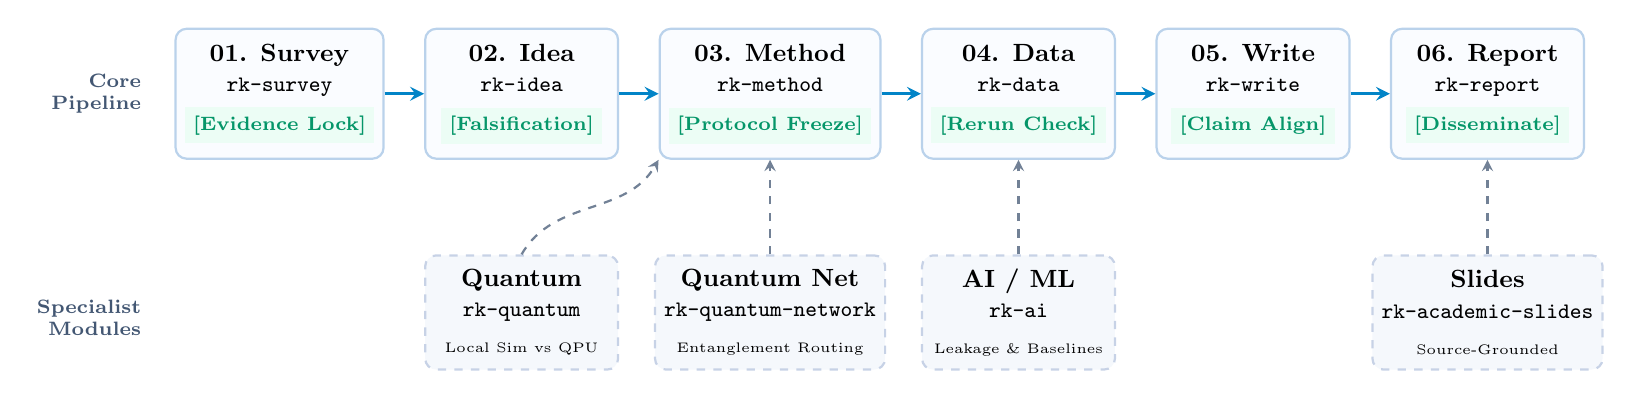
\begin{tikzpicture}[
  >=stealth,
  node distance=0.6cm and 0.5cm,
  stage/.style={
    draw=boxborder,
    fill=lightfill,
    rounded corners=4pt,
    thick,
    minimum width=2.45cm,
    minimum height=1.65cm,
    align=center,
    font=\small
  },
  specialist/.style={
    draw=specborder,
    fill=specfill,
    dashed,
    rounded corners=4pt,
    thick,
    minimum width=2.45cm,
    minimum height=1.45cm,
    align=center,
    font=\small
  }
]

  % Core Pipeline
  \node[stage] (s1) at (0, 0) {\textbf{01. Survey}\\\texttt{\footnotesize rk-survey}\\[3pt]\colorbox{gatebg}{\textcolor{gatecolor}{\scriptsize\bfseries [Evidence Lock]}}};
  \node[stage, right=of s1] (s2) {\textbf{02. Idea}\\\texttt{\footnotesize rk-idea}\\[3pt]\colorbox{gatebg}{\textcolor{gatecolor}{\scriptsize\bfseries [Falsification]}}};
  \node[stage, right=of s2] (s3) {\textbf{03. Method}\\\texttt{\footnotesize rk-method}\\[3pt]\colorbox{gatebg}{\textcolor{gatecolor}{\scriptsize\bfseries [Protocol Freeze]}}};
  \node[stage, right=of s3] (s4) {\textbf{04. Data}\\\texttt{\footnotesize rk-data}\\[3pt]\colorbox{gatebg}{\textcolor{gatecolor}{\scriptsize\bfseries [Rerun Check]}}};
  \node[stage, right=of s4] (s5) {\textbf{05. Write}\\\texttt{\footnotesize rk-write}\\[3pt]\colorbox{gatebg}{\textcolor{gatecolor}{\scriptsize\bfseries [Claim Align]}}};
  \node[stage, right=of s5] (s6) {\textbf{06. Report}\\\texttt{\footnotesize rk-report}\\[3pt]\colorbox{gatebg}{\textcolor{gatecolor}{\scriptsize\bfseries [Disseminate]}}};

  \draw[->, very thick, paperblue] (s1) -- (s2);
  \draw[->, very thick, paperblue] (s2) -- (s3);
  \draw[->, very thick, paperblue] (s3) -- (s4);
  \draw[->, very thick, paperblue] (s4) -- (s5);
  \draw[->, very thick, paperblue] (s5) -- (s6);

  % 4 Specialist modules placed under s2, s3, s4, s6
  \node[specialist, below=1.2cm of s2] (e1) {\textbf{Quantum}\\\texttt{\footnotesize rk-quantum}\\[2pt]\tiny Local Sim vs QPU};
  \node[specialist, below=1.2cm of s3] (e2) {\textbf{Quantum Net}\\\texttt{\footnotesize rk-quantum-network}\\[2pt]\tiny Entanglement Routing};
  \node[specialist, below=1.2cm of s4] (e3) {\textbf{AI / ML}\\\texttt{\footnotesize rk-ai}\\[2pt]\tiny Leakage \& Baselines};
  \node[specialist, below=1.2cm of s6] (e4) {\textbf{Slides}\\\texttt{\footnotesize rk-academic-slides}\\[2pt]\tiny Source-Grounded};

  \draw[->, thick, dashed, draw=navy!60] (e1.north) to[out=60, in=-120] (s3.south west);
  \draw[->, thick, dashed, draw=navy!60] (e2.north) -- (s3.south);
  \draw[->, thick, dashed, draw=navy!60] (e3.north) -- (s4.south);
  \draw[->, thick, dashed, draw=navy!60] (e4.north) -- (s6.south);

  % Side Labels
  \node[font=\scriptsize\bfseries, text=navy!80, anchor=east, align=right] at ($(s1.west)+(-0.3,0)$) {Core\\Pipeline};
  \node[font=\scriptsize\bfseries, text=navy!80, anchor=east, align=right] at ($(s1.west)+(-0.3,-2.85)$) {Specialist\\Modules};

\end{tikzpicture}
\end{document}
